\chapter{Diseño}
\section{Diseño general de la aplicación}
Para todo el conjunto de la aplicación se va a hacer uso del lenguaje javascript. En el lado del cliente, haremos uso del estándar ES6 de javascript, lo cual nos permitirá una programación orientada a objetos. En el servidor también se hace uso del mismo lenguaje, pero dejaremos de lado la programación orientada a objetos.

Empezando por el backend su estructura es simple. Nos encontramos con una serie de rutas, unos modelos, una serie de \glspl{middleware} y el servidor propiamente dicho. El funcionamiento será el siguiente: Mantendremos un servidor de Express corriendo sobre Node, dicho servidor estará conectado con una base de datos de Mongo y con PaperTrail, cuando reciba una petición, esta pasará por los middleware que realizarán una serie de tratamientos, como por ejemplo la verificación de la autenticación. Una vez hecho esto, según la ruta requerida, se llegará a una función y dicha función hará la consulta pertinente y devolverá los datos.

En el frontend, tenemos un diseño un tanto más complejo. Dispondremos de una web HTML, en la que existe una ruta al archivo Javascript donde estará definida toda la aplicación. La aplicación se compone de un archivo client.js, que podría considerarse la clase principal, y una serie de componentes, que según la ruta, y el funcionamiento de react-router-dom, serán inyectados. La aplicación mantendrá un estado global, del que se nutrirán todos los componentes, según la filosofia Redux. Entre los componentes podremos distinguir entre dos tipos, los componentes "StateFull", que son los que serán conocedores del estado de la aplicación y contendrá lógica, y los "React Stateless Functional Components" que simplemente reciben datos y los muestran.


Para estructurar las carpetas, aunque no hay un estándar definido, nuestra decisión ha sido la mostrada en las imágenes \ref{fig:frontend} \ref{fig:backend}.

\begin{figure}
  \begin{center}
    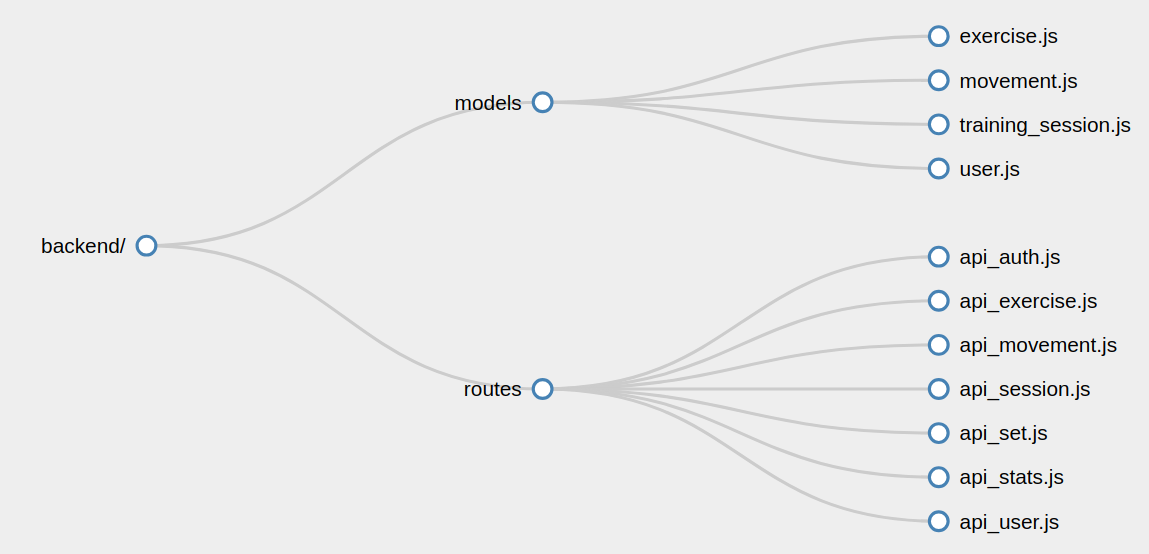
\includegraphics[width=\textwidth]{imagenes/backend.png}
    \caption{Estructura backend}
    \label{fig:backend}
  \end{center}
\end{figure}

\begin{figure}
  \begin{center}
    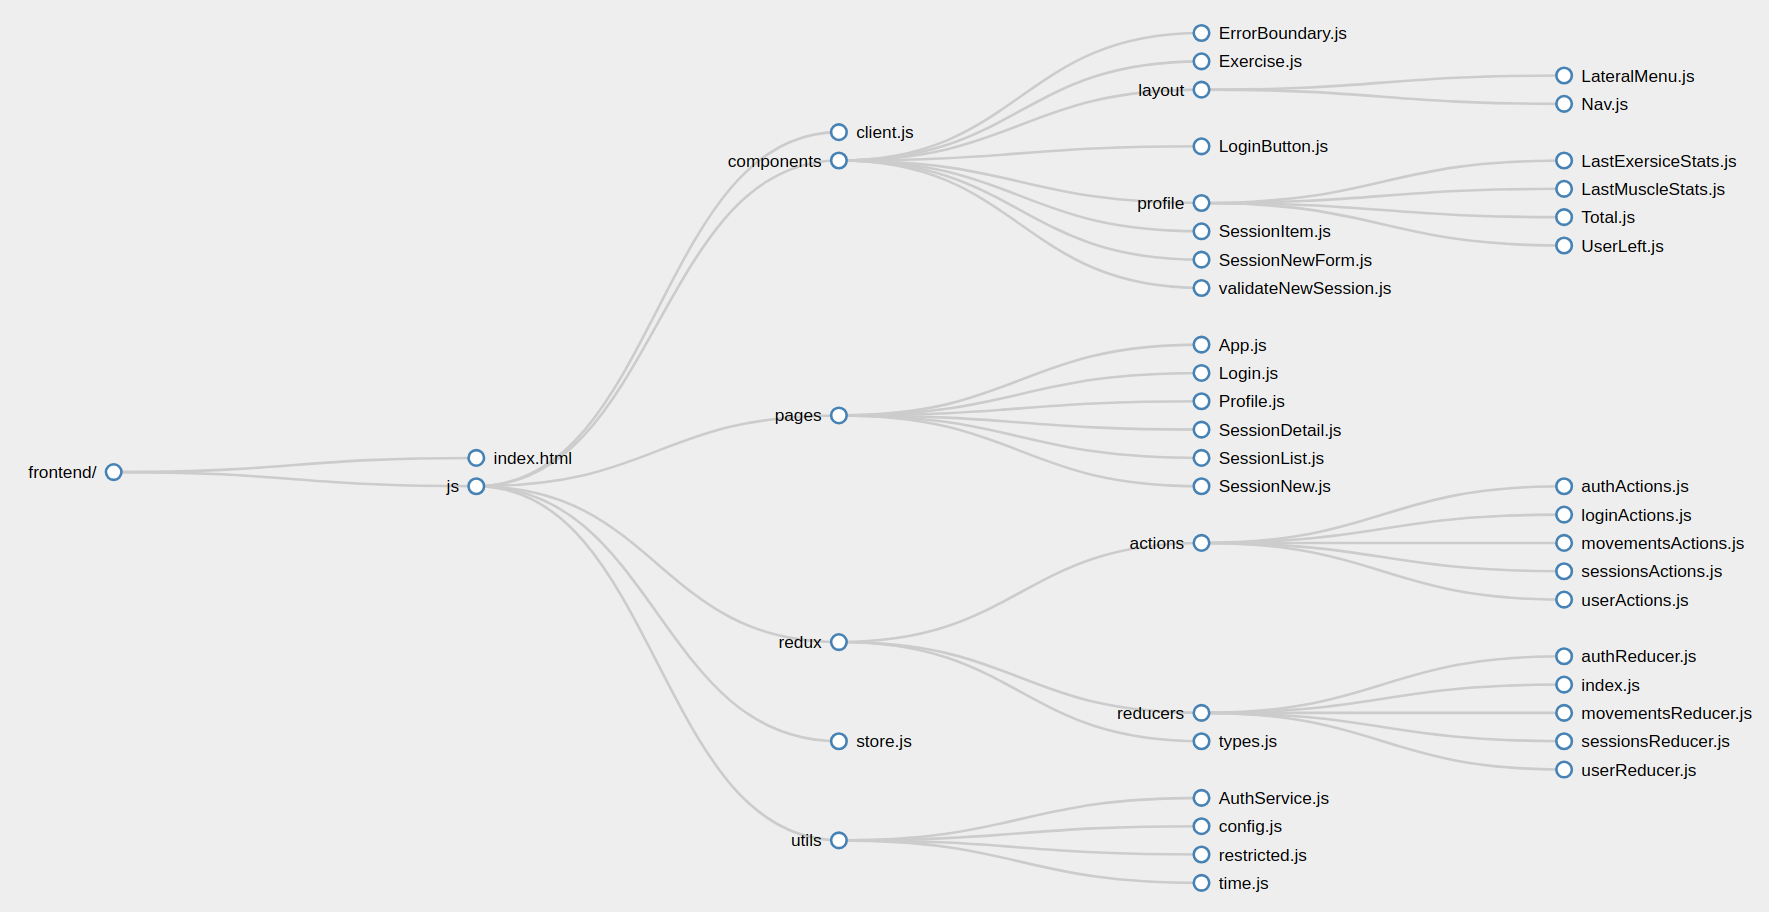
\includegraphics[width=\textwidth]{imagenes/frontend.png}
    \caption{Estructura frontend}
    \label{fig:frontend}
  \end{center}
\end{figure}


\section{Desarrollo colaborativo}
Este proyecto se sustenta en el uso de software libre, software el cual se puede obtener, usar e incluso modificar de forma libre. Y siendo este proyecto del mismo carácter, cabe destacar el uso de soluciones para el desarrollo colaborativo de software. En este caso hemos hecho uso de \Gls{git} en la plataforma GitHub. Aunque en este proyecto solo existe un desarrollador, la filosofía de Git sigue siendo muy útil, ya que nos permite realizar un control de versiones y por lo tanto nos da la oportunidad de llevar una traza de la evolución del proyecto y la posibilidad de volver atrás en caso necesario. Además permite la creación de ramas, gracias a la cual, el hecho se desarrollar y testear nuevas funcionalidades sin afectar al proyecto principal se hace mucho más simple, y por otro lado permite el uso de programas como GreenKeeper \ref{fig:greenkeeper}, que crea automáticamente nuevas ramas para poder testear las últimas versiones de nuestras dependencias.

\begin{figure}
  \begin{center}
    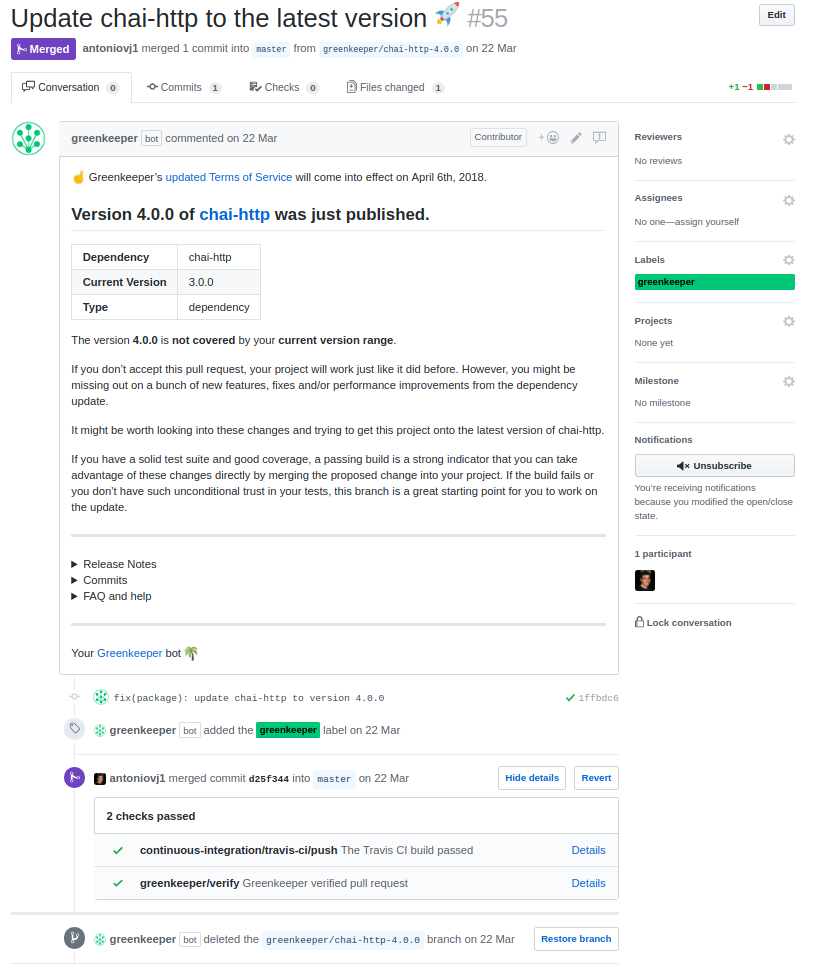
\includegraphics[width=\textwidth]{imagenes/greenkeeper.png}
    \caption{Ejemplo ejecución GreenKeeper}
    \label{fig:greenkeeper}
  \end{center}
\end{figure}

Además hemos llevado a cabo una metodología de desarrollo DevOps, en la cual no se distingue entre el desarrollo del software y su administración, es decir el desarrollo se integra con la administración, se crea una nueva funcionalidad y se testea su despliegue, todo como un proceso conjunto.

\section {Tests (Unitarios y Cobertura)}
Para poder llevar a cabo una metodología DevOps, nos apoyamos en un desarrollo guiado por pruebas, o Test-Driven Development. Dichas pruebas, serán implementadas mediante test unitarios, y nos servirán para comprobar que cada nueva actualización en el código no genera errores en otras partes.

Gracias esta forma de desarrollo, no aseguramos que toda la funcionalidad que se va añadiendo a la aplicación funciona de la forma esperada, y gracias a ello podemos tener la seguridad de que el despliegue de las nuevas versiones no causan ningún tipo de problema.

En esta ocasión, los test unitarios, serán tests basados en comportamiento, es decir, la forma de evaluar su éxito o fracaso, es comprobando si el resultado de una determinada solicitud, es el que esperábamos o no. Por ejemplo, para comprobar si una llamada al \gls{endpoint} de la API que devuelve un usuario dada una ID, el test consistirá en verificar que el estado de la petición es 200, y que el nombre del usuario que es devuelto, es justo el que habíamos solicitado.


Además de los test unitarios, disponemos de los test de cobertura, que en este caso gracias a Jest, son exactamente los mismos. Este tipo de test consiste en evaluar qué porcentaje del código y que posibles críticas han sido testeadas. Este es importante ya que si la cobertura es muy baja o alguna de las casuísticas importantes no ha sido testeada, no podemos tener total confianza en los tests, y por lo tanto necesitaremos desarrollar más, para verificar estas partes no cubiertas.

Todo este trabajo se va a desarrollar haciendo uso de Jest, una plataforma de tests de Facebook, que nos permitirá realizar todo tipo de test, tanto unitarios como de cobertura, incluyendo funciones avanzadas para el testeo de React con datos falsos "Mocks"


\section {Integración continua}


La integración continua (CI - Continuous integration) consiste en verificar que cada vez que añadimos un cambio al código este no rompe el comportamiento de la aplicación o de alguna parte de esta. Teniendo en cuenta que hacemos uso de un entorno colaborativo, y que en el futuro puede haber múltiples desarrolladores, esto cobra una vital importancia.

Para llevar a cabo la integración continua, haremos uso de los tests unitarios comentados anteriormente, lo que nos ayudará a evitar errores y mantener la calidad del código.

El procedimiento para llevar a cabo la integración continua, se ejecutará a través de Travis CI. Travis CI, es una plataforma que tras ser configurada, monitorizará nuestro repositorio de GitHub, y con cada nuevo push o \gls{pull request} a este, se encargará de ejecutar los test unitarios y verificar si todo sigue funcionando de una forma adecuada. En caso de que no sea así, Travis CI nos notificará, en incluso podrá evitar que se realice un \gls{merge}.


\section {Despliegue continuo}
Una vez que siguiendo los pasos anteriores, podemos estar seguros de que todo esta en perfecto estado, llega el momento de desplegar los cambios introducidos.
En este caso vamos a realizar los despliegues de forma automática, es decir, cada vez que modificamos código en el repositorio, y dichos cambios pasan los test de Travis CI, será desplegados.

Para el despliegue continuo  (CD - Continuous deployment) haremos uso de Heroku. Una vez configurada la plataforma, monitorizará el estado de nuestro repositorio y de los test, y será capaz de generar nuevas builds y despliegues de forma automática.

Cabe destacar que esta herramienta nos brinda la posibilidad de volver a despliegues antiguos, ya que aunque todos los tests se hayan ejecutado con éxito, siempre queda la posibilidad de que exista algún comportamiento inesperado y por lo tanto será útil volver atrás mientras solucionamos los problemas.

\section {Provisionamiento}

Además de la forma de despliegue anterior, se proporcionará la posibilidad de realizar despliegues en la nube de Google.

Este proceso consiste en la creación y configuración de las máquinas virtuales para poder usar nuestra aplicación. Es decir, la instalación de todo el software adicional necesario y la configuración de este.

En este caso vamos a hacer uso de Vagrant y Ansible, el primero ejecutará la tarea de la creación de las máquinas en la nube de Google, el segundo se encargará del aprovisionamiento propiamente dicho, ya que mediante su archivo de configuración conocido como playbook, instalará todo el software necesario, lo configurará, descargara el repositorio de Git y finalmente lo pondrá en funcionamiento.










